\section{Evidence}

\begin{figure}[t]
  \centering
  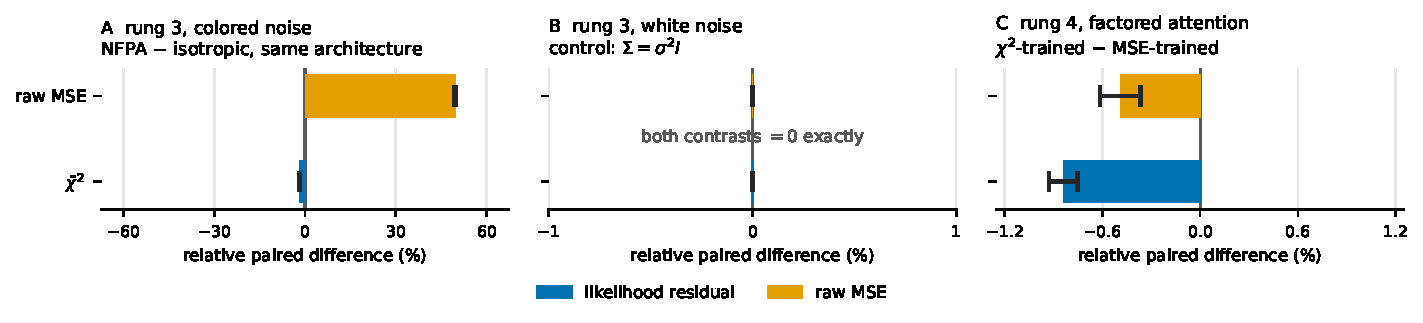
\includegraphics[width=\linewidth]{figures/evidence}
  \caption{\textbf{A}, rung 3: the reversal and its replication. Relative paired
  differences, NFPA minus the isotropic baseline; solid = frozen ten seeds,
  hatched = an independent twenty-seed replication. The metrics point in
  \emph{opposite} directions --- the reversal --- and the cohorts agree.
  Symmetric-log axis (the effects differ by over an order of magnitude);
  cohorts are never pooled. \textbf{B}, what the factors recover at the
  separable condition: the channel subspace almost exactly, the temporal one
  only weakly. Generated from archived summaries.}
  \label{fig:evidence}
\end{figure}

\paragraph{NFPA under channel compression.}
Rung 3 is consolidated at $C=8>k_c=2$ channels, matched rank $k=k_ck_t=6$: NFPA, an isotropically trained factored baseline of the same architecture, CW-PCA, and PCA on the same seeds (superseded rung-2 evidence and the TIDMAD diagnostics motivating the lift are in Appendix~\ref{app:protocol}). NFPA and the isotropic baseline differ only in the training metric, isolating it. It reverses: in the frozen ten-seed experiment NFPA is better under the likelihood residual ($-0.0192$, 95\% interval $[-0.0194,-0.0190]$) and worse under raw MSE ($+0.0034$, $[+0.0034,+0.0034]$), both excluding zero. An independent twenty-seed replication of the identical configuration agrees in sign and magnitude ($-0.0190$, $[-0.0192,-0.0189]$; $+0.0034$, $[+0.0034,+0.0034]$); cohorts are reported separately, any pooled figure being post-hoc rather than a thirty-seed confirmatory experiment. Against unrestricted CW-PCA the residual differs by $-0.0026$ ($[-0.0026,-0.0025]$) --- finite-sample, not evidence the Kronecker restriction is superior. The twenty-seed white-noise run is an identity check: at $\Sigma=\sigma^2I$ the objectives coincide up to scale, and its exact zero shows the pipeline adds no spurious contrast. Estimating the covariance from $2{,}048$ noise-only calibration events preserves the reversal in all ten seeds ($-0.0191$, $[-0.0193,-0.0189]$; $+0.0034$), degrading NFPA's likelihood residual and raw MSE by $0.0078\%$ and $0.0345\%$ of its own oracle held-out values --- consistent with invariance to a global whitening scale and an accurately estimated covariance \emph{shape}, but one fixed condition, not a robustness sweep (Table~\ref{tab:round10}). \looseness=-1

\paragraph{Rung 4 (exploratory): the metric in a factored-attention network.}
One factored-attention architecture is trained on the TIDMAD readout under two objectives differing only in the metric --- \texttt{T-mse} on the unwhitened spectrogram, \texttt{T-chi2} on the $\Sigma^{-1}$-weighted residual --- at matched data, budget and evaluation grid, at two independent seeds. \emph{The reversal does not appear at either seed.} The $\Sigma^{-1}$-trained arm is better on \emph{both} criteria in both runs: held-out paired differences $-1.15$ and $-1.17\times10^{-4}$ on the likelihood residual, $-57.2$ and $-57.4$ on raw MSE, the latter opposite to prediction; all four signs agree across seeds, which bounds run-to-run variation rather than characterising it. The release's coarse score does not separate the arms ($-1.0\times10^{-3}$; window and file-block intervals both span zero), and both arms sit far below the published baselines (Appendix~\ref{app:rung4-baselines}). A degenerate metric would explain it, and we tested for one: $J$ spans a factor $441$ and the whitening weights have coefficient of variation $0.69$, the same order as the rung-3 geometry where the reversal \emph{is} observed ($1.10$; white control $0$). The metric is comparably non-degenerate at both rungs, so the absence is a property of this instantiation, not of the ladder. \looseness=-1

\paragraph{What the covariance-weighted factors recover.}
The metric also changes what the representation \emph{is}. At the separable condition NFPA recovers the planted channel subspace almost exactly ($0.035$ projector error against the isotropic $1.021$) while temporal recovery stays weak ($0.768$ against $1.280$) --- an asymmetry a joint number would hide. All seven paired contrasts --- projector errors and held-out decoding of amplitude, rise time and decay time --- favour NFPA, every seed-level interval excludes zero, and all ten seeds agree in sign. No recovery threshold was predeclared, so these are continuous estimates, not a verdict (Appendix~\ref{app:protocol}).

\paragraph{Transfer of the noise model.}
On a public gravitational-wave strain release \citep{gwoscgw150914,macleod2021gwpy}, a whitened score matching its reference form to $10^{-12}$ and calibrated on synthetic stationary noise (dispersion $1.15$) is seven to nine times over-dispersed on real H1 and L1 strain ($9.42$, $8.83$; leave-one-out $1.77$, $7.29$). A covariance model can be correctly implemented, validated synthetically, and still fail to transfer: implementation identity is not calibration, and transfer is where a learned geometry is falsified.
